%% 
%% Copyright 2007-2024 Elsevier Ltd
%% 
%% This file is part of the 'Elsarticle Bundle'.
%% ---------------------------------------------
%% 
%% It may be distributed under the conditions of the LaTeX Project Public
%% License, either version 1.3 of this license or (at your option) any
%% later version.  The latest version of this license is in
%%    http://www.latex-project.org/lppl.txt
%% and version 1.3 or later is part of all distributions of LaTeX
%% version 1999/12/01 or later.
%% 
%% The list of all files belonging to the 'Elsarticle Bundle' is
%% given in the file `manifest.txt'.
%% 
%% Template article for Elsevier's document class `elsarticle'
%% with numbered style bibliographic references
%% SP 2008/03/01
%% $Id: elsarticle-template-num.tex 249 2024-04-06 10:51:24Z rishi $
%%
\documentclass[preprint,12pt]{Definitions/elsarticle}
\usepackage{mathtools}
\usepackage{float} 
\usepackage{relsize}
\usepackage{xcolor}
\usepackage{caption}
\usepackage{placeins}
\usepackage{geometry}
\usepackage{tabularx}
\usepackage{bigints}

\graphicspath{ {./Figures/} }

\newcommand{\mb}{\mathbf}
\newcommand{\tn}{\textnormal}
\newcommand{\unit}[1]{\ensuremath{\, \mathrm{#1}}}

\newcommand{\bmz}{\mbox{\boldmath $z$\unboldmath}}
\newcommand{\bmr}{\mbox{\boldmath $r$\unboldmath}}
\newcommand{\bmb}{\mbox{\boldmath $b$\unboldmath}}
\newcommand{\bms}{\mbox{\boldmath $s$\unboldmath}}
\newcommand{\bmg}{\mbox{\boldmath $g$\unboldmath}}
\newcommand{\bmq}{\mbox{\boldmath $q$\unboldmath}}
\newcommand{\bmU}{\mbox{\boldmath $U$\unboldmath}}
\newcommand{\bmu}{\mbox{\boldmath $u$\unboldmath}}
\newcommand{\bmv}{\mbox{\boldmath $v$\unboldmath}}
\newcommand{\bmw}{\mbox{\boldmath $w$\unboldmath}}
\newcommand{\bmm}{\mbox{\boldmath $m$\unboldmath}}
\newcommand{\bmi}{\mbox{\boldmath $i$\unboldmath}}
\newcommand{\bmj}{\mbox{\boldmath $j$\unboldmath}}
\newcommand{\bmk}{\mbox{\boldmath $k$\unboldmath}}
\newcommand{\bmx}{\mbox{\boldmath $x$\unboldmath}}
\newcommand{\bmX}{\mbox{\boldmath $X$\unboldmath}}
\newcommand{\bmH}{\mbox{\boldmath $H$\unboldmath}}
\newcommand{\bmy}{\mbox{\boldmath $y$\unboldmath}}
\newcommand{\bmn}{\mbox{\boldmath $n$\unboldmath}}
\newcommand{\bmf}{\mbox{\boldmath $f$\unboldmath}}
\newcommand{\bmF}{\mbox{\boldmath $F$\unboldmath}}
\newcommand{\bmS}{\mbox{\boldmath $S$\unboldmath}}
\newcommand{\bmG}{\mbox{\boldmath $G$\unboldmath}}
\newcommand{\bmV}{\mbox{\boldmath $V$\unboldmath}}
\newcommand{\bmI}{\mbox{\boldmath $I$\unboldmath}}
\newcommand{\bmD}{\mbox{\boldmath $D$\unboldmath}}
\newcommand{\bmnu}{\mbox{\boldmath $\nu$\unboldmath}}

\newcommand{\DefTen}{\mathbb{D}}
\newcommand{\EyeTen}{\mathbb{I}}

\newcommand{\MVBcmnt}[1]{{\color{red}{\em #1}}}

%\newcolumntype{L}[1]{>{\raggedright\let\newline\\\arraybackslash\hspace{0pt}}m{#1}}
%\newcolumntype{C}[1]{>{\centering\let\newline\\\arraybackslash\hspace{0pt}}m{#1}}
%\newcolumntype{R}[1]{>{\raggedleft\let\newline\\\arraybackslash\hspace{0pt}}m{#1}}

\newcommand{\parD}[2]{\frac{\partial #1}{\partial #2}}
\newcommand{\parDD}[2]{\frac{\partial^2 #1}{\partial #2^2}}
\newcommand{\norm}[1]{\left\lVert#1\right\rVert}

%% Use the option review to obtain double line spacing
%% \documentclass[authoryear,preprint,review,12pt]{elsarticle}

%% Use the options 1p,twocolumn; 3p; 3p,twocolumn; 5p; or 5p,twocolumn
%% for a journal layout:
%% \documentclass[final,1p,times]{elsarticle}
%% \documentclass[final,1p,times,twocolumn]{elsarticle}
%% \documentclass[final,3p,times]{elsarticle}
%% \documentclass[final,3p,times,twocolumn]{elsarticle}
%% \documentclass[final,5p,times]{elsarticle}
%% \documentclass[final,5p,times,twocolumn]{elsarticle}

%% For including figures, graphicx.sty has been loaded in
%% elsarticle.cls. If you prefer to use the old commands
%% please give \usepackage{epsfig}

%% The amssymb package provides various useful mathematical symbols
\usepackage{amssymb}
%% The amsmath package provides various useful equation environments.
\usepackage{amsmath}
%% The amsthm package provides extended theorem environments
%% \usepackage{amsthm}

%% The lineno packages adds line numbers. Start line numbering with
%% \begin{linenumbers}, end it with \end{linenumbers}. Or switch it on
%% for the whole article with \linenumbers.
%% \usepackage{lineno}

\journal{Journal of Computational Physics}

\begin{document}

\begin{frontmatter}

%% Title, authors and addresses

%% use the tnoteref command within \title for footnotes;
%% use the tnotetext command for theassociated footnote;
%% use the fnref command within \author or \affiliation for footnotes;
%% use the fntext command for theassociated footnote;
%% use the corref command within \author for corresponding author footnotes;
%% use the cortext command for theassociated footnote;
%% use the ead command for the email address,
%% and the form \ead[url] for the home page:
%% \title{Title\tnoteref{label1}}
%% \tnotetext[label1]{}
%% \author{Name\corref{cor1}\fnref{label2}}
%% \ead{email address}
%% \ead[url]{home page}
%% \fntext[label2]{}
%% \cortext[cor1]{}
%% \affiliation{organization={},
%%             addressline={},
%%             city={},
%%             postcode={},
%%             state={},
%%             country={}}
%% \fntext[label3]{}

\title{Coupling the Level Set Method to Moments and Particles for Computing N-phase flows with phase change.}

%% use optional labels to link authors explicitly to addresses:
%% \author[label1,label2]{}
%% \affiliation[label1]{organization={},
%%             addressline={},
%%             city={},
%%             postcode={},
%%             state={},
%%             country={}}
%%
%% \affiliation[label2]{organization={},
%%             addressline={},
%%             city={},
%%             postcode={},
%%             state={},
%%             country={}}

\author{} %% Author name

%% Author affiliation
\affiliation{organization={},%Department and Organization
            addressline={}, 
            city={},
            postcode={}, 
            state={},
            country={}}

%% Abstract
\begin{abstract}
A new algorithm that hybridizes marker particles with the coupled level set moment-of-fluid method to improve the interface reconstruction in N-phase flow problems is proposed. This approach uses both near and on-interface Lagrangian marker particles to improve the slope reconstruction for the multimaterial moment of fluid (MOF) method. Deriving the MOF slopes from particles overcomes the surface tension checkerboard instability of the MOF method, first discussed by Ye et al. (2023).  Ye et al. developed the Continuous Moment of Fluid (CMOF) method in order to overcome this checkerboard instability. The coupled particle moment of fluid method (PMOF) method proposed herein is compared to both MOF and CMOF on rigid body tests and multiphase flow problems in 2D, axisymmetric ``R-Z", and 3D coordinate systems. Examples include two and three material multiphase flows, with and without phase change: bubble formation, liquid lens dynamics, freezing droplet on a cold substrate, and an impinging liquid jet on vapor ullage in a cryogenic tank. It has been found that augmenting the interface representation with meshless particle produces similar results to that of the CMOF method, at a computational cost similar to that of MOF. The proposed method is volume-preserving and generalizable to unstructured grids.
\end{abstract}

%%Graphical abstract
%\begin{graphicalabstract}
%\includegraphics{grabs}
%\end{graphicalabstract}

%%Research highlights
%\begin{highlights}
%\item Research highlight 1
%\item Research highlight 2
%\end{highlights}

%% Keywords
\begin{keyword}
%% keywords here, in the form: keyword \sep keyword
Moment-of-Fluid (MOF)
\sep Level Set
\sep Particles
\sep Surface tension
\sep Phase change
\sep Multimaterial
\sep Multiphase
\sep N-phase flow

%% PACS codes here, in the form: \PACS code \sep code

%% MSC codes here, in the form: \MSC code \sep code
%% or \MSC[2008] code \sep code (2000 is the default)

\end{keyword}

\end{frontmatter}

%% Add \usepackage{lineno} before \begin{document} and uncomment 
%% following line to enable line numbers
%% \linenumbers

%% main text
%%

%% Use \section commands to start a section
%\section{Example Section}
%\label{sec1}
%% Labels are used to cross-reference an item using \ref command.

%Section text. See Subsection \ref{subsec1}.

%% Use \subsection commands to start a subsection.
%\subsection{Example Subsection}
%\label{subsec1}

%Subsection text.

%% Use \subsubsection, \paragraph, \subparagraph commands to 
%% start 3rd, 4th and 5th level sections.
%% Refer following link for more details.
%% https://en.wikibooks.org/wiki/LaTeX/Document_Structure#Sectioning_commands

%\subsubsection{Mathematics}
%% Inline mathematics is tagged between $ symbols.
%This is an example for the symbol $\alpha$ tagged as inline mathematics.

%% Displayed equations can be tagged using various environments. 
%% Single line equations can be tagged using the equation environment.
%\begin{equation}
%f(x) = (x+a)(x+b)
%\end{equation}

%% Unnumbered equations are tagged using starred versions of the environment.
%% amsmath package needs to be loaded for the starred version of equation environment.
%\begin{equation*}
%f(x) = (x+a)(x+b)
%\end{equation*}

%% align or eqnarray environments can be used for multi line equations.
%% & is used to mark alignment points in equations.
%% \\ is used to end a row in a multiline equation.
%\begin{align}
% f(x) &= (x+a)(x+b) \\
%      &= x^2 + (a+b)x + ab
%\end{align}

%\begin{eqnarray}
% f(x) &=& (x+a)(x+b) \nonumber\\ %% If equation numbering is not needed for a row use \nonumber.
%      &=& x^2 + (a+b)x + ab
%\end{eqnarray}

%% Unnumbered versions of align and eqnarray
%\begin{align*}
% f(x) &= (x+a)(x+b) \\
%      &= x^2 + (a+b)x + ab
%\end{align*}

%\begin{eqnarray*}
% f(x)&=& (x+a)(x+b) \\
%     &=& x^2 + (a+b)x + ab
%\end{eqnarray*}

%% Refer following link for more details.
%% https://en.wikibooks.org/wiki/LaTeX/Mathematics
%% https://en.wikibooks.org/wiki/LaTeX/Advanced_Mathematics

%% Use a table environment to create tables.
%% Refer following link for more details.
%% https://en.wikibooks.org/wiki/LaTeX/Tables
%\begin{table}[t]%% placement specifier
%% Use tabular environment to tag the tabular data.
%% https://en.wikibooks.org/wiki/LaTeX/Tables#The_tabular_environment
%\centering%% For centre alignment of tabular.
%\begin{tabular}{l c r}%% Table column specifiers
%% Tabular cells are separated by &
%  1 & 2 & 3 \\ %% A tabular row ends with \\
%  4 & 5 & 6 \\
%  7 & 8 & 9 \\
%\end{tabular}
%% Use \caption command for table caption and label.
%\caption{Table Caption}\label{fig1}
%\end{table}


%% Use figure environment to create figures
%% Refer following link for more details.
%% https://en.wikibooks.org/wiki/LaTeX/Floats,_Figures_and_Captions
%\begin{figure}[t]%% placement specifier
%% Use \includegraphics command to insert graphic files. Place graphics files in 
%% working directory.
%\centering%% For centre alignment of image.
%\includegraphics{example-image-a}
%% Use \caption command for figure caption and label.
%\caption{Figure Caption}\label{fig1}
%% https://en.wikibooks.org/wiki/LaTeX/Importing_Graphics#Importing_external_graphics
%\end{figure}
\section{Introduction}
\textcolor{red}{add table: existing multiphase flow MOF methods with surface tension, report curvature algorithm}
%does curvature discretization in conjunction with MOF exhibit checkerboard instability?

\noindent\makebox[\textwidth]{
\begin{tabularx}{1.25\textwidth}{|l|c|c|l|l|}
	\hline
	Authors   & Curvature       & N-phase & Interface      & grid \\ 
		      & Discretization  &         & Representation &      \\ \hline
	Kumaran et al. 2024 \cite{KUMARAN2024} & height function & 2 & sharp & staggered, unstructured\\
	Pan et al. 2024 \cite{PAN2024} & height function & 2 & sharp, front tracking & staggered, structured\\
	Mukundan et al. 2020 \cite{mukundan2020MOF}  & Level Set  & 2 & sharp & staggered, structured \\
	Li et al. 2015\cite{LiETAL2015IncompressibleMultiphase} & height function & $\geq 2$ & sharp & staggered, structured \\
	\hline
\end{tabularx}
}


\begin{table}[H]
	\small
	\centering
	\caption{Recent Multimaterial MOF papers and their curvature discretizations.}
	\renewcommand{\arraystretch}{1.2} 
	\begin{tabular}{|l|l|l|l|l|}
		\hline
		Authors   & Curvature Discretization  & N-phase & Interface Representation & grid \\ \hline
		Kumaran et al. CITE &  & &  \\
		Mukundan et al. 2020 \cite{mukundan2020MOF}  & Level Set  & &  \\
		Li et al.\cite{LiETAL2015IncompressibleMultiphase} & Height Function & &  \\
		\hline
	\end{tabular}
	\label{curvaturediscretization_comparison}
\end{table}
%Add Popinet Edge Based, Interface Representation (diffuse/sharp),staggered or collocated

\FloatBarrier
\section{Mathematical Model}
	\begin{align}
		\phi_{m_\textrm{rigid}}(\mb{x},t) &= \left\{
		\begin{array}{ll}
			> 0 & \mb{x} \in \tn{material}\,\: m_\textrm{rigid}, \\ 
			\leq 0 & \tn{otherwise},
		\end{array}
		\right.\\
		\phi_{m_\textrm{fluid}}(\mb{x},t) &= \left\{
		\begin{array}{ll}
			> 0 & \mb{x} \in \tn{material}\,\: m_\textrm{fluid}\cup m_\textrm{fluid,ghost}, \\ 
			\leq 0 & \tn{otherwise}.
		\end{array}
		\right.
	\end{align}

	\begin{equation}
	\phi_{m_1,m_2}(\mb{x},t) = \left\{
	\begin{array}{ll}
	> 0 & \mb{x} \in \tn{material}\,\: m_1, \\ 
	< 0 & \mb{x} \in \tn{material}\,\: m_2, \\ 
	= 0 & \tn{for }\mb{x}\,\: \tn{along}\,\:(m_1,m_2)\,\:\tn{interface}. \\ 
	\end{array}
	\right.
	\end{equation}
	
The multiphase system is comprised of $M_{\textrm{fluid}}$ deforming materials and $M_{\textrm{rigid}}$ non-deforming materials. The fluid materials tessellate the entire computational domain (extended through any rigid bodies), and where a material $m_{\textrm{fluid}}$ intersects with a solid $m_{\textrm{rigid}}$ region, the governing equations for the rigid body is used. In regions not containing a $m_{\textrm{rigid}}$, the incompressible Navier-Stokes equations of immiscible flows govern the fluid materials.

\section{Governing Equations} \label{governingeqs}
\subsection{Multimaterial Level Sets}
\noindent We define the rigid and fluid materials using the following multimaterial level set formulation:
\begin{equation}
\phi_{m_\textrm{rigid}}(\bmx,t) = \left\{
\begin{array}{ll}
> 0 & \bmx \in \tn{material}\,\: m_\textrm{rigid}, \\ 
\leq 0 & \tn{otherwise},
\end{array}
\right.
\end{equation}
\begin{equation}
\phi_{m_\textrm{fluid}}(\bmx,t) = \left\{
\begin{array}{ll}
> 0 & \bmx \in \tn{material}\,\: m_\textrm{fluid}\cup m_\textrm{fluid,ghost}, \\ 
\leq 0 & \tn{otherwise}.
\end{array}
\right.
\end{equation}
For position vector $\bmx$ and time $t$. Material $m_\textrm{rigid}$ is defined as the region where $\phi_{m_\textrm{rigid}}>0$ and the domain of material $m_\textrm{fluid}$ as the region where $\phi_{m_\textrm{fluid}}>0$ and $\phi_{m_\textrm{rigid}}<0$. $m_\tn{ghost}$ indicates the region in which the fluid level set is extended through the rigid body. This extension is implemented as in \cite{ArientiSussman2014embedded} in which the fluid interface is extended orthogonally to the rigid body, regardless of contact angle. This configuration can be seen in figure \ref{fig:LSextend} below.\\

\begin{figure}[htbp]
	\centering
	\includegraphics[width=0.45\textwidth]{LSextend.eps}
	\caption{fluid level set extension through rigid region}
	\label{fig:LSextend}
\end{figure}

\noindent The interface level set, $\phi_{m1,m2}$,
represents the interface between materials
$m_1$ and $m_2$
\begin{equation}
\phi_{m_1,m_2}(\bmx,t) = \left\{
\begin{array}{ll}
> 0 & \bmx \in \tn{material}\,\: m_1, \\ 
< 0 & \bmx \in \tn{material}\,\: m_2, \\ 
= 0 & \tn{for }\bmx\,\: \tn{along}\,\:(m_1,m_2)\,\:\tn{interface}. \\ 
\end{array}
\right.
\end{equation}
The interfacial level sets are not stored nor extended through the material level sets as in \cite{yeETAL2023CMOF}. Where needed, we instead obtain the interfacial level sets from the involved material level sets as
\begin{equation}
\phi_{m_1,m_2} = \frac{\phi_{m_1}-\phi_{m_2}}{2}.
\end{equation}
The associated normal $\bmn$ and curvature $\kappa$ for the level set functions are defined as
\begin{equation}
\bmn_{m_1,m_2} = 
\frac{\nabla \phi_{m_1,m_2}}{||\nabla \phi_{m_1,m_2}||}, \hspace{10pt}   
\kappa_{m_1,m_2} = 
\nabla \cdot \frac{\nabla \phi_{m_1,m_2}}{||\nabla \phi_{m_1,m_2}||}.
\end{equation}


\subsection{Conservation of mass}
\noindent Each fluid material, $m_\tn{fluid}$, is assumed to be incompressible, 
so that the velocity field $\bmu$ is divergence free within each fluid material:
\begin{equation}
\label{eq:cnt}
\nabla \cdot \bmu = 0.
\end{equation}
The following conditions on $\nabla \cdot \bmu$ are enforced to account for phase change and any mass sources or sinks:
\begin{equation}
\nabla \cdot \bmu = 
\sum_{\tn{sources}} 
\frac{\dot{m}_{\tn{source}}}
{\rho_{\tn{source}}}\delta(\phi_{m_{\tn{source}}}) -
\sum_{\tn{sinks}} 
\frac{\dot{m}_{\tn{sink}}}
{\rho_{\tn{sink}}}\delta(\phi_{m_{\tn{sink}}}) 
\label{eq:divu}
\end{equation}
\noindent where $\delta(\phi)$ is the Dirac delta function,
\begin{equation}
\delta(\phi)=H'(\phi)
\end{equation}
\noindent and $H(\phi)$ is the Heaviside function,
\begin{align}
H(\phi)=\left\{ \begin{array}{cc}
1 & \phi>0  \\
0 & \phi\le 0. \end{array} 
\right.
\end{align}
\noindent $\dot{m}$ is the mass flux. For the mass flux of boiling 
liquid across the liquid/vapor interface, we have
\begin{equation}
\dot{m} = 
\frac{k_{l}\nabla T_{l}\cdot \bmn_{l,v} - 
	k_{v}\nabla T_{v}\cdot \bmn_{l,v}}{L},
\label{eq:massflux}
\end{equation}
where
$k_{l}$ and $k_{v}$ are the respective thermal conductivities of the 
liquid and ambient vapor regions. $\rho_{l}$ and
$\rho_{v}$ are the respective densities of the liquid and ambient vapor
regions. $L$ is the latent heat of vaporization. Vector $\bmn_{l,v}$ is the interface normal that points from the vapor region into the liquid,
\begin{equation}
\bmn_{l,v} = \frac{\nabla\phi_{l,v}}{||\nabla\phi_{l,v}||}.
\end{equation}


\subsection{Conservation of momentum:}
\noindent For each material in its domain $\phi_{m}(\bmx,t)>0$ we have the following conservation of momentum:
\begin{align}
(\bmu\rho_{m})_{t}+
\nabla\cdot(\bmu \otimes \bmu \rho_{m}+p_{m} \EyeTen)=
\nabla\cdot(2\mu_{m}\DefTen)+
\rho_{m}\bmg (1-\alpha_{m}(T_{m}-T_{0m})).
\label{eq:NS}
\end{align}
with density $\rho_{m}$, pressure $p_{m}$, temperature $T_{m}$, coefficients of thermal expansion $\alpha_{m}$, and viscosities $\mu_{m}$ for material $m$. $\bmg$ is the acceleration due to gravity and $\DefTen= \frac{1}{2}(\nabla\bmu+(\nabla\bmu)^{T})$ is the rate of deformation tensor. 


\subsection{Conservation of energy:} 
\noindent For each material in its domain $\phi_{m}(\bmx,t)>0$ we have the conservation of energy equation:
\begin{equation}
\label{eq:heat}
(\rho_{m}C_{p,m}T_{m})_t+
\nabla\cdot(\bmu\rho_{m}C_{p,m}T_{m})=
\nabla\cdot ( k_{m}\nabla T_{m}).
%\hspace{10pt} \tn{if} \hspace{10pt} \phi_{m}(\bmx,t)>0,
\end{equation}
$C_{p,m}$ is the heat capacity, $k_{m}$ is the thermal conductivity, and $T_{m}$ is the temperature corresponding to material $m$. 


\subsection{Interfacial jump conditions:}
\noindent We represent a deforming interface undergoing phase change with the following general equations.
\begin{eqnarray}
\phi_{m_{s},m_{d}} + 
\bmu_{m_{s}}\cdot\nabla\phi_{m_{s},m_{d}} =
-\frac{\dot{m}}{\rho_{s}}||\nabla\phi_{m_{s},m_{d}}||
\end{eqnarray}
\begin{eqnarray}
\phi_{m_{d},m_{s}} + 
\bmu_{m_{s}}\cdot\nabla\phi_{m_{d},m_{s}} =
\frac{\dot{m}}{\rho_{s}}||\nabla\phi_{m_{d},m_{s}}||
\end{eqnarray}
Or, equivalently:
\begin{eqnarray}
\phi_{m_{s},m_{d}} + 
\bmu_{m_{d}}\cdot\nabla\phi_{m_{s},m_{d}} =
-\frac{\dot{m}}{\rho_{d}}||\nabla\phi_{m_{s},m_{d}}||
\end{eqnarray}
\begin{eqnarray}
\phi_{m_{d},m_{s}} + 
\bmu_{m_{d}}\cdot\nabla\phi_{m_{d},m_{s}} =
\frac{\dot{m}}{\rho_{d}}||\nabla\phi_{m_{d},m_{s}}||
\end{eqnarray}
For the level set $\phi_{m_{s},m_{d}}$ indicating the interface separating a material $m_{s}$ region from a
material $m_{d}$ region.
$m_{s}$ is defined as the material id associated with a `source' material 
and $m_{d}$ is the corresponding `destination' material (e.g. for boiling, $m_s$ is the liquid material and $m_d$ the vapor region and for freezing, $m_s$ would indicate the liquid material and $m_d$ the icing material). \\

\noindent For the velocity, pressure, 
and temperature interface jump conditions between materials $m_{s}$ and $m_{d}$, we apply the following definitions:
\begin{align}
\bmu_{m_{s}}\cdot \bmn_{m_{s},m_{d}}-
\bmu_{m_{d}}\cdot \bmn_{m_{s},m_{d}} &= 
\dot{m}\bigg(\frac{1}{\rho_{m_{d}}}-
\frac{1}{\rho_{m_{s}}}\bigg),\\
(p_{m_{s}}\EyeTen-
p_{m_{d}}\EyeTen)\cdot\bmn_{m_{s},m_{d}} &=
-\sigma_{m_{s},m_{d}}\kappa_{m_{s},m_{d}}\bmn_{m_{s},m_{d}} \\
&\qquad + (2\mu_{m_{s}}\DefTen_{m_{s}}-
2\mu_{m_{d}}\DefTen_{m_{d}})\cdot\bmn_{m_{s},m_{d}},\nonumber\\
T_{m_{s}} &= T_{m_{d}}.
\label{vtp_jump}
\end{align}
Where $\sigma_{m_{s},m_{d}}$ is the prescribed surface tension and $\kappa_{m_{s},m_{d}}$ is the interface curvature, defined as
\begin{equation}
\kappa_{m_{s},m_{d}}=\nabla\cdot
\frac{\nabla\phi_{m1,m2}}
{||\nabla\phi_{m1,m2}||}.
\end{equation}

\subsection{Triple point junction}
\noindent At a triple point, a three-phase equilibrium (Neumann's triangle \cite{de2013capillarity}) determines the contact angles for a steady state, dependent on the surface tension of the phases in contact. (see Figure \ref{fig:triple_point}(a)):
\begin{equation}
\label{eq:triple_point_eqlib}
\frac{\sin(\theta_{1})}{\sigma_{23}}=
\frac{\sin(\theta_{2})}{\sigma_{13}}=
\frac{\sin(\theta_{3})}{\sigma_{12}}.
\end{equation}
\newline


\FloatBarrier
\section{Numerical Method}
\FloatBarrier
\subsection{Interface Reconstruction}
\FloatBarrier
\subsubsection{Moment-of-Fluid reconstruction}
\begin{figure}[H]
	\centering
	\includegraphics[width=0.85\textwidth]{triple_point_drop_impact.eps}
	\caption{(\textbf{a}) Physical Domain, shown here for a triple point. The contact angles $\theta$ are determined at equilibrium by the surface tension forces $\sigma$.  \\
		(\textbf{b}) Discretized Domain. $\times$ : cell centers, $\bullet$ : cell centroids, $\scriptstyle \blacksquare$ : MAC velocities}
	\label{fig:triple_point}
\end{figure}   
\unskip
\begin{figure}[H]
	\centering
	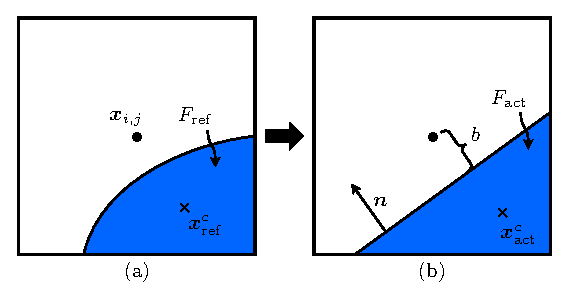
\includegraphics[width=0.77\textwidth]{mof_reconstruction.eps}
	\caption{(\textbf{a}) Material domain in a cell $\Omega_{i,j}$, a single phase shown in blue corresponding with reference volume $F_\tn{ref}$ and centroid $\bmx_\tn{ref}^c$.  \\
		(\textbf{b}) The piecewise linear MOF reconstruction. The line segment for the reconstructed volume can be represented as $\Omega_{i,j}\cap\{\bmx|\bmn\cdot(\bmx-\bmx_{i,j})+b=0\}$. }
	\label{fig:mof_reconstruction}
\end{figure}   
\unskip
\begin{figure}[H]
	\centering
	\includegraphics[width=0.8\textwidth]{mof_tes.eps}
	\caption{MOF reconstruction, volume-tessellation (nested dissection) procedure. Points indicate centroids, white space is the unoccupied region, and zones of color indicate reconstructed materials.}
	\label{fig:mof_tess}
\end{figure}   

\FloatBarrier
\subsubsection{Continuous MOF reconstruction}
\begin{figure}[H]
	\centering
	\includegraphics[width=0.5\textwidth]{CMOFcentroid.eps}
	\caption{CMOF reconstruction.
		Black dots represent cell centroids, blue dots represent 
		`material 1' centroids, and the red dot represents the CMOF supercell (red boundary)
		centroid associated with the center cell (green boundary) for `material 1'. \\
		The CMOF
		reconstructed interface (solid red line inside the center cell) is found such that it is the line
		segment which minimizes the difference between the CMOF reference 
		centroid (red dot) and the CMOF derived centroid (centroid associated
		with the dashed red line) subject to the constraint that
		the reference MOF volume fraction (`material 1' volume fraction within the 
		center cell) equals the actual CMOF reconstructed
		volume fraction (`material 1' volume fraction below the solid red line in the center cell).
		\label{CMOFstencil} }
\end{figure}   

\FloatBarrier
\subsubsection{Particle Level Set MOF reconstruction}
\begin{figure}[H]
	\centering
	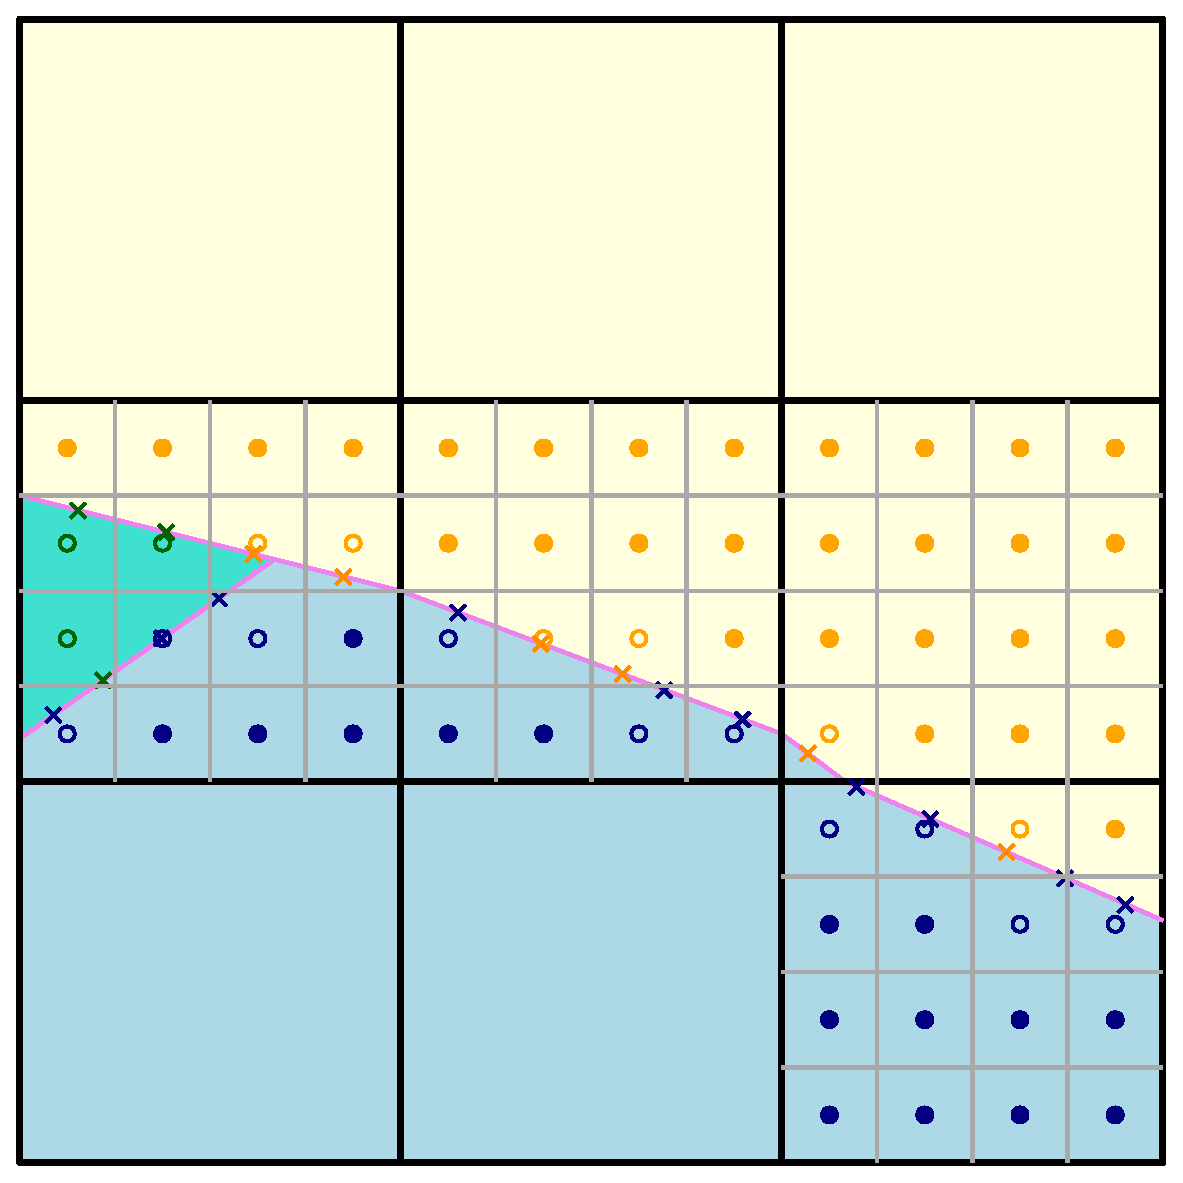
\includegraphics[width=0.65\textwidth]{particleseeding_particles2.eps}
	\caption{subdividing cell, $N=4$, grid lines: $\Delta x_\tn{sub}$. $\bullet$ : near-interface particles, $\times$ : on-interface particles, $\bigcirc$ : cell-centers for particle sent to interface, color indicates associated material}
	\label{fig:particleseeding}
\end{figure}   

\subsection{Redistancing}
\begin{figure}[H]
	\includegraphics[width=0.95\textwidth]{redistancing.eps}
	\caption{MOF redistancing procedure (shown for candidate cell-center $\times$ in update cell I).\\
		(\textbf{a}) Candidate distances (black dotted lines) are measured from the center of update cell (I) to the center, corners, and faces of the support cell (II). In this configuration, the nearest sample point coinciding with a different material is indicated by the red dotted line. If the material interface coincides with the cell boundary, this gives the exact distance.\\
		(\textbf{b}) The distance between update cell (I) using the reconstructed normal for the interface in support cell (II) is shown by the red dotted line. Since the intersection point is contained within the support cell, the two material ids are obtained using test points (white dots) on both sides. In this example, the signed distance and corresponding normal vector for the red material level set, green material level set, and red-green interface level sets are updated. Note: The candidate normal distance with support cell (III) is shown by the black dotted line. Since the intersection point is not contained within the support cell, this distance is not accepted.\\
		(\textbf{c}) The distance between update cell (I) and the material intersections in support cell (II) is measured (red dotted line). Test points (white dots)around the triple point are used to find the material ids. In this example, the red, blue, and green material level sets are updated and the red-blue, red-green, and blue-green interface level sets are updated. Similarly for the red-green-yellow triple point.\\
		(\textbf{d}) Distances between update cell (I) and the cell face intersections in support cell(II) is shown. Test points and level set updates follow as in (c). In this example, red and blue material level sets and blue-red interface level sets are updated (black dotted line) and similarly for red and green.}
	\label{fig:MOFredistancing}
\end{figure}   
\unskip
\begin{figure}[H]
	\centering
	\includegraphics[width=0.7\textwidth]{redistancing_3Dfixed.png}
	\caption{3D MOF redistancing. Update cell (left), querying normal distances to potential nearest interface plane intersection (black dashed line) within support cell (right) as well as distances to the line formed by the intersection of the interface plane with the cell boundaries.}
	\label{fig:redistancing_3D}
\end{figure}   
\unskip
\begin{figure}[H]
	\centering
	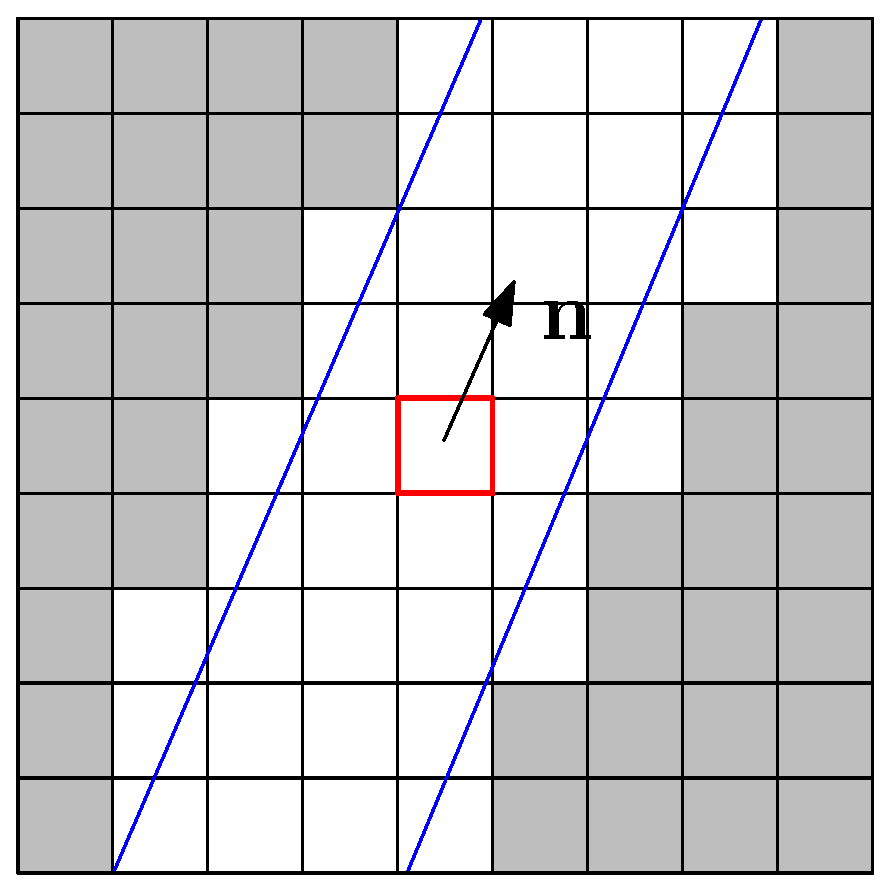
\includegraphics[width=0.5\textwidth]{reduced_stencil.eps}
	\caption{The reduced neighborhood stencil. The red cell indicates a support cell about which we construct a $9\times9(\times9)$ update neighborhood. The blue lines indicate the reduced band (3cells thick), aligned in the direction of the interface normal. The grey regions indicate the parts of the $9\times9(\times9)$ stencil that lie outside the narrow band reduction that are not evaluated. If the normal is oriented with the grid, the neighborhood stencil is reduced to a $3\times9(\times3)$ region.}
	\label{fig:reducedstencil}
\end{figure}   
\unskip
\begin{figure}[H]
	\centering
	\includegraphics[width=0.65\textwidth]{stencilgap.eps}
	\caption{The maximum extent of the stencil-covered region of each piecewise linear interface segment is indicated by the dashed lines. At the end of the linear segments, the update region does not extend the full thickness of the narrow band due to the orientation of the stencils. This may produce regions for which cells are within the narrow band but not updated during the redistancing step. This can seen at the junctions of the linear segments (a small gap off the left junction and a larger one on the right, the red circle is centered at a junction with the radius indicating the width of the narrow band). Directly near the end of the linear segment, cells are still guaranteed to be updated due to the stencil thickness, but further away, regions may form in which cells do not get redistanced. Since the cells in the gap region that lie farther from the interface are not updated, the error from these may pollute the level set function and therefore eventually the slopes and volume fractions. However, in practice the error introduced is found to be negligible and the speedup from the stencil reduction significant. In addition to remaining sufficiently accurate, this reduction does not affect the linearity preserving property of the reconstruction (the method is exact for piecewise linear interfaces).}
	\label{fig:stencilorientation}
\end{figure}   

\FloatBarrier
\subsection{Staggered Grid Projection Method}
Outline of the operator-split staggered grid projection method:
\begin{enumerate}
	\item Find the time step $\Delta t=t^{n+1}-t^{n}$:
	\begin{equation}
	\begin{dcases}
	\Delta t_{1}&=\mathlarger{\mathlarger{\min}}_{d=1,\ldots,\tn{dim}}
	\frac{\min \Delta x_{d}}{2 (dim) \max||u_{d}^{n}||} \\	
	\Delta t_{2}&=\mathlarger{\mathlarger{\min}}_{d=1,\ldots,\tn{dim}}
	\frac{\min\Delta x_{d}}{(dim)\max||u_{d}^{\tn{phase change},n-1}||} \\
	\Delta t_{3}&=\mathlarger{\mathlarger{\min}}_{d=1,\ldots,\tn{dim}} \quad
	\mathlarger{\mathlarger{\min}}_{m_1,m_2=1,\ldots,M}
	\Delta x_{d}^{3/2}
	\sqrt{\frac{\rho_{m_1}+\rho_{m_2}}
		{2\pi\sigma_{m_1,m_2}}} 
	\end{dcases}
	\label{stiffconstraint}
	\end{equation}
	\begin{equation}
	\Delta t = \tn{CFL} \min(\Delta t_{1},\Delta t_{2},\Delta t_{3})
	\end{equation}
	where `dim' is the dimension of the problem ($2$ or $3$). We let the coefficient `$\tn{CFL}$' $= \frac{1}{2}$. The time step is restricted by the CFL conditions on the MAC velocity, the rate of phase change, and surface tension.\\




\par\noindent
Ghost Fluid Method for surface tension \cite{kang2000boundary}:
\begin{eqnarray*}
\frac{p_{I,L}-p_{L}}{\rho_{L}\theta_{L}\Delta x}=
\frac{p_{R}-p_{I,R}}{\rho_{R}\theta_{R}\Delta x}
\end{eqnarray*}

% gas on left  liquid on right  normal=+1 (liquid level set) \kappa>0
\begin{eqnarray*}
p_{I,R}-p_{I,L}=-\sigma\kappa 
\end{eqnarray*}

\begin{eqnarray*}
\frac{p_{I,R}+\sigma\kappa-p_{L}}{\rho_{L}\theta_{L}\Delta x}=
\frac{p_{R}-p_{I,R}}{\rho_{R}\theta_{R}\Delta x}
\end{eqnarray*}

\begin{eqnarray*}
p_{I,R}\left( 
\frac{1}{\rho_{L}\theta_{L}\Delta x}+
\frac{1}{\rho_{R}\theta_{R}\Delta x} \right)=
\frac{p_{L}}{\rho_{L}\theta_{L}\Delta x}+
\frac{p_{R}}{\rho_{R}\theta_{R}\Delta x}-
\frac{\sigma\kappa}{\rho_{L}\theta_{L}\Delta x}
\end{eqnarray*}

\begin{eqnarray*}
\rho_{f}\equiv \rho_{L}\theta_{L}+\rho_{R}\theta_{R}
\end{eqnarray*}

\begin{eqnarray*}
p_{I,R}\rho_{f}=
p_{L}\rho_{R}\theta_{R}+
p_{R}\rho_{L}\theta_{L}-\sigma\kappa\rho_{R}\theta_{R}
\end{eqnarray*}

\begin{eqnarray*}
\frac{p_{R}\rho_{f}-p_{I,R}\rho_{f}}{\rho_{f}\rho_{R}\theta_{R}\Delta x}=
\end{eqnarray*}
\begin{eqnarray*}
\frac{p_{R}\rho_{R}\theta_{R}-p_{L}\rho_{R}\theta_{R}+
 \sigma\kappa\rho_{R}\theta_{R}}{\rho_{f}\rho_{R}\theta_{R}\Delta x}=
\end{eqnarray*}
\begin{eqnarray*}
\frac{p_{R}-p_{L}}{\rho_{f}\Delta x}+\sigma\kappa\frac{1}{\rho_{f}\Delta x}
\end{eqnarray*}
Assume
\begin{eqnarray*}
|\kappa|<\frac{1}{\Delta x},
\end{eqnarray*}
then we want:
\begin{eqnarray*}
\left(\Delta t \sigma\frac{1}{\rho_{f}\Delta x^{2}}\right)\Delta t \le 
\frac{1}{2}\Delta x
\end{eqnarray*}
\begin{eqnarray*}
\Delta t \le \Delta x^{3/2} \sqrt{\frac{\rho_{f}}{2\sigma}}
\end{eqnarray*}

\par\noindent
Slope reconstruction using level set function, particles, centroid and
volume fraction:
\begin{eqnarray*}
 \phi(\vec{x})=\vec{n}\cdot(\vec{x}-\vec{x}_{0})+b
\end{eqnarray*}
\begin{eqnarray*}
(\vec{n},b)=\mbox{argmin}
 \sum_{ijk}\delta(||\vec{x}_{ijk}-\vec{x}^{c}||)
 (\phi(\vec{x}_{ijk})-\phi_{ijk})^{2}+
 \sum_{p}\delta(||\vec{x}_{p}-\vec{x}^{c}||)
 (\phi(\vec{x}_{p})-\phi_{p})^{2}
\end{eqnarray*}

	\subsection{Cell Integrated Semi-Lagrangian}\label{CISL}
	The following Cell Integrated Semi-Lagrangian (CISL) procedures are implemented and terms discretized as in \cite{pei2019hierarchical, LiETAL2015IncompressibleMultiphase,VAHAB2021}. This method follows an operator-splitting approach. The steps listed below are solved by the conservative  Weymouth and Yue \cite{WeymouthYue2010conservative}, or alternatively, the Euler Implicit-Lagrange Explicit (EI-LE) \cite{scardovelli2003interface,aulisa2007DirSplit} directionally-split methods. 
	
	The idea behind the CISL integration is to trace the characteristics backwards of a cell being updated using in an unconditionally stable Semi-Lagrangian manner \cite{STRAIN1999semiLagrangian, wang2012hybrid}. From this a `departure' region is constructed and mapped back to the cell and the containing volume fraction and centroid reconstructed for the updated time. For the mapping function and full CISL algorithm, the reader is referred to \cite{LiETAL2015IncompressibleMultiphase}. The CISL-MOF reconstruction is visualized in Fig. \ref{fig:cisl_mass} for a single direction. The discretizations used for the CISL algorithm are provided below.
	
	\item Directionally split CISL-MOF, advection of the volume fractions and centroids\\
	For materials $m=1, \ldots, M$,
	\begin{equation}
	F_{m,t}+\nabla\cdot(\bmu F_{m})=0
	\end{equation}
	\begin{equation}
	\bmx_{m,t}^c=\bmu(\bmx_{m}^c)
	\end{equation}
	\begin{equation}
	F_{m,(i,j,k)}^{n+1}=
	\frac{\bigintss_{\Omega_{i,j,k}^{Depart}} \chi_m^{n}(\bmx)d\bmx }
	{||\Omega_{i,j,k}^\tn{Depart}||} 		
	\end{equation}
	\begin{equation}
	\bmx_{m,(i,j,k)}^{c,n+1}=
	\frac{\bigintss_{\mathcal{T}_\tn{CISL}(\Omega_{m,(i,j,k)}^\tn{Depart})} 
		\bmx\chi_m^{n}(\mathcal{T}_\tn{CISL}^{-1}(\bmx)) d\bmx}
	{||\mathcal{T}_\tn{CISL}(\Omega_{m,(i,j,k)}^{Depart})||}
	\end{equation}
	Where $\displaystyle \chi_m$ is defined as a characteristic function such that $\chi_m(\bmx) = 1$ if $\bmx \in \Omega_{m,(i,j,k)}$, $0$ otherwise. $\mathcal{T}_\tn{CISL}$ represents the mapping function. Refer to Figure \ref{fig:cisl_mass} for integration over the region of the backwards-traced characteristics.
	
	\item CISL level set advection
	\begin{equation}
	\phi_{m,t}+\bmu\cdot\nabla\phi_{m}=0, \hspace{10pt} 
	m=1,\ldots,M 
	\end{equation}
	\begin{equation}
	\phi_{m,(i,j,k)}^{n+1}=
	\frac{\bigintss_{\Omega_{m,(i,j,k)}^\tn{Depart}} \phi_m^{n}(\bmx) d\bmx}
	{||\Omega_{i,j,k}^\tn{Depart}||}
	\end{equation}
	\item CISL advection of the MAC velocity 
	\begin{equation}
	(\rho \bmu)_{t}+\nabla\cdot(\rho\bmu\bmu)=0, \label{advection}
	\end{equation}
	\begin{equation}
	u_{i-1/2,j,k}^{n+1}=
	\frac{\bigintss_{\Omega_{i-1/2,j,k}^\tn{Depart}}
		\sum_{m=1}^{M} \rho_{m}\chi_m^{n}(\bmx)u^{n}(\bmx) d\bmx}
	{\bigintss_{\Omega_{i-1/2,j,k}^\tn{Depart}}
		\sum_{m=1}^{M} \rho_{m}\chi_m^{n}(\bmx) d\bmx}
	\end{equation}
	\begin{equation}
	v_{i,j-1/2,k}^{n+1}=
	\frac{\bigintss_{\Omega_{i,j-1/2,k}^\tn{Depart}}
		\sum_{m=1}^{M} \rho_{m}\chi_m^{n}(\bmx)v^{n}(\bmx) d\bmx}
	{\bigintss_{\Omega_{i,j-1/2,k}^\tn{Depart}}
		\sum_{m=1}^{M} \rho_{m}\chi_m^{n}(\bmx) d\bmx}
	\end{equation}
	\begin{equation}
	w_{i,j,k-1/2}^{n+1}=
	\frac{\bigintss_{\Omega_{i,j,k-1/2}^\tn{Depart}}
		\sum_{m=1}^{M} \rho_{m}\chi_m^{n}(\bmx)w^{n}(\bmx) d\bmx}
	{\bigintss_{\Omega_{i,j,k-1/2}^\tn{Depart}}
		\sum_{m=1}^{M} \rho_{m}\chi_m^{n}(\bmx) d\bmx}
	\end{equation}
	
	\begin{figure}[h!]
		\centering
		\includegraphics[width=0.95\textwidth]{fig_3_cisl.png}
		\caption{CISL-MOF method [figure from \cite{pei2019hierarchical}], shown here for $x$-direction for the blue material.\\
			(a) Reconstructed MOF interface and centroids at departure time $t^n$ for slab of cells [\{i-1, i, i+1\},j] and target cell $\Omega_{i,j}^\tn{target}$ at arrival time $t^n+\Delta t$.\\
			(b) Characteristics are traced backwards and CISL mapping function $T^\tn{CISL}$ calculated.\\
			(c) The CISL mapping function sends the material from the departure time to the update time and its intersection with the target cell is found.\\
			(d) The contained region is combined to obtain the volume fraction and centroid}
		\label{fig:cisl_mass}
	\end{figure}
	
	\item CISL temperature advection (liquid and gas materials)
	\begin{equation}
	(\rho_{m} C_{p,m} T_{m})_{t}+
	\nabla\cdot(\rho_{m} C_{p,m} \bmu T_{m})=0, \hspace{10pt}
	m=1,\ldots,M \label{adv2}
	\end{equation}
	
	\item Directionally split particle advection (2nd order Runge-Kutta)
	\begin{equation}
	\bmx_{p,t}=\bmu(\bmx_{p})
	\end{equation}
\end{enumerate}
\subsection{Phase Change} \label{Phase Change}
To ensure mass conservation, it is necessary that the motion of the interface remain consistent with the mass flux across the interface. The relevant steps are outlined below, implemented from \cite{VAHAB2021}.
\begin{enumerate}
	\item Redistribution of mass source (the mass flux $\dot{m}$ is redistributed form source material $m_{s}$ to destination material $m_d$): Eq. \ref{eq:massflux}. This is implemented as follows
	\begin{itemize}
		\item Loop through the grid, for every cell that has a valid closest point map, find if it changes phase at the corresponding closest point. 
		\item If it does, then $\dot{m}$ is found:
		\item $\dot{m} = \bigg[\frac{k\nabla T\cdot \bmn}{L}\bigg]$ 
	\end{itemize}
	
	\item Phase change velocity (from source material $m_{s}$ to destination material $m_{d}$).
	\begin{equation}
	\bmu^{\tn{phase change}}=-\frac{\dot{m}}{\rho_{m_{d}}}\bmn_{m_{d}}, \bigg(\tn{ or } \bmu^{\tn{phase change}}=\frac{\dot{m}}{\rho_{m_{s}}}\bmn_{m_{s}}\bigg)
	\label{uphasechange}
	\end{equation}
	\item Phase change, level set unsplit advection
	\begin{equation}
	\phi_{m,t}+\bmu^{\tn{phase change}}\cdot\nabla\phi_{m}=0,
	\qquad m=m_{s} \mbox{ or } m_{d}.
	\end{equation}
	\item Phase change: unsplit CISL advection
	\begin{equation}
	F_{m,t}+\nabla\cdot(\bmu^{\tn{phase change}}F_{m})=0,
	\qquad m=m_{s} \mbox{ or } m_{d}.
	\end{equation}
	\begin{equation}
	\bmx_{m,t}^c=\bmu^\tn{phase change}(\bmx_{m}^c)
	\end{equation}
	
	\item Unsplit particle advection for phase change (1st order Forward Euler)
	\begin{equation}
	\frac{d\bmx_{p}}{dt}=\bmu^\tn{phase change}(\bmx_{p})
	\end{equation}
	
	
	\item Thermal diffusion
	\begin{equation}
	\frac{(\rho C_{p,m})^{\tn{mix},n+1}}{\Delta t^{\tn{swept}}}
	(T^{n+1}_{m}-T_{\tn{sat},m})=
	\nabla\cdot (k_{m} \nabla T^{n+1}_{m})
	\label{diffusion1}
	\end{equation}
	This large sparse matrix system is solved using the multigrid preconditioned conjugate gradient (MGPCG) method. (See figure \ref{fig:tempgrad} for the temperature gradient). Note: The temperature is stored at corresponding material centroids; as the interface shifts during phase change, a crossing time approach is used to interpolate the temperature from the old time to new centroids.\cite{liu2022novel,VAHAB2021}
	\item Viscosity
	\begin{equation}
	\frac{\rho^{\tn{mix},n+1}}{\Delta t}
	(\bmu^{\ast}-\bmu^{\tn{advection}})=
	\nabla\cdot(2\mu\DefTen^{\ast})-
	\rho^{n+1}(\alpha^{n+1}(T^{n+1}-T_{0}))\bmg
	\label{diffusion3}
	\end{equation}
	An implicit solver is used for the viscous term $\nabla\cdot(2\mu\DefTen^{\ast})$. In this case, BiCGSTAB using a Jacobi preconditioner and red-black Gauss-Seidel smoother.
	\item Pressure projection
	The pressure projection step is formulated using Chorin's method \cite{chorin1968numerical}. From the momentum equation, we have
	\begin{equation}
	\frac{\bmu^{n+1}-\bmu^{\ast}}{\Delta t}=
	-\frac{\nabla p^{n+1}}{\rho^{\tn{MAC,mix},n+1}}+\bmg-
	\frac{\sum_{m=1}^{M} \gamma_{m}\kappa_{m}\nabla H(\phi_{m})}
	{\rho^{\tn{MAC,mix},n+1}}
	\label{pressuregrad}
	\end{equation}
	On the right hand side are the viscous force, gravitational force, and surface tension force terms, respectively. Note: the surface tension force term is handled in a ghost fluid manner \cite{fedkiw1999GFM,sussman2007sharp}. Remark: This equation exhibits a very strong discontinuity at the triple point (in which both $\nabla H$ and $\kappa_m$ behave as delta functions, proportional to $1/\Delta x$, this is further exacerbated once the divergence is taken (Eq. \ref{eq:pressureproj}) and the whole term gains a large error proportional to $1/\Delta x^3$. However, similarly as in \cite{BukacETAL2023diffuse} (for an error proportional to $1/\Delta x$), it is found that since this error is localized just at the triple point, it hasn't been observed to affect the behavior away from the triple point. In the numerical experiments, the $\kappa_m$ discontinuity converges under grid refinement (future convergence studies are warranted).  \\
	
	Taking the divergence of both sides, 
	\begin{equation}
	\frac{1}{\Delta t} \bigg(\nabla \cdot \bmu^{n+1} - \nabla\cdot\bmu^{\ast}\bigg) = \nabla\cdot \bigg[-\frac{\nabla p^{n+1}}{\rho^{\tn{MAC,mix},n+1}}+\bmg-
	\frac{\sum_{m=1}^{M} \gamma_{m}\kappa_{m}\nabla H(\phi_{m})}
	{\rho^{\tn{MAC,mix},n+1}}\bigg]
	\label{eq:pressureproj}
	\end{equation}
	From equation \ref{eq:divu}, we enforce the expansion term
	\begin{equation}
	\nabla \cdot \bmu^{n+1} = 
	\sum_{\tn{sources}} 
	\frac{\dot{m}_{\tn{source}}}
	{\rho_{\tn{source}}}\delta(\phi_{m_{\tn{source}}}) -
	\sum_{\tn{sinks}} 
	\frac{\dot{m}_{\tn{sink}}}
	{\rho_{\tn{sink}}}\delta(\phi_{m_{\tn{sink}}}) 
	\end{equation}
	%% remember: \kappa_{m1}=-\kappa_{m2}, H(\phi_{m1})=1-H(\phi_{m2})
	and use the following $\gamma_m$:
	\begin{equation}
	\gamma_{m_1}=\gamma_{m_2}=\frac{1}{2} \sigma_{m_1,m_2}
	\end{equation}
	for two materials $m1$, $m2$ in a $3\times 3(\times 3)$ local stencil. If three materials $m1$, $m2$, $m3$, are present in the stencil, then the following terms are used instead (satisfying Eq. \ref{eq:triple_point_eqlib}):
	\begin{equation}
	\gamma_{m_1}=\frac{1}{2} (\sigma_{m_1,m_2}+\sigma_{m_1,m_3}-\sigma_{m_2,m_3})
	\end{equation}
	\begin{equation}
	\gamma_{m_2}=\frac{1}{2} (\sigma_{m_1,m_2}+\sigma_{m_2,m_3}-\sigma_{m_1,m_3})
	\end{equation}
	\begin{equation}
	\gamma_{m_3}=\frac{1}{2} (\sigma_{m_1,m_3}+\sigma_{m_2,m_3}-\sigma_{m_1,m_2})
	\end{equation}
	Equation \ref{eq:pressureproj} can then be solved for the pressure term. BiCGSTAB using a multigrid preconditioner and red-black Gauss-Seidel smoother is used.\\
	The velocity for the next timestep is then
	\begin{equation}
	\bmu^{n+1} = \bmu^{\ast}-\Delta t\frac{\nabla p^{n+1}}{\rho^{\tn{MAC,mix},n+1}}
	\end{equation}
\end{enumerate}

\begin{figure}[h!]
	\centering
	\includegraphics[width=0.5\textwidth]{vahab_probept.PNG}
	\caption{[figure from \cite{VAHAB2021}] \\
		The closest point is found on the interface by $x_\tn{closest}=x_{i,j}-\phi_{m_1,m_2}\bmn_{m_1,m_2}$,\\
		two probe points are extended in either normal direction and $T(x_\tn{probe})$ is found by interpolation.\\
		$\nabla T_{m_1}=(T_{\tn{probe},m_1}-T_{\tn{sat},m_1,m_2})\bmn_{m_1,m_2}/h$ and 
		$\nabla T_{m_2}=-(T_{\tn{probe},m_2}-T_{\tn{sat},m_1,m_2})\bmn_{m_1,m_2}/h$, where $T_\tn{sat}$ is the phase change saturation temperature.
	}
	\label{fig:tempgrad}
\end{figure}

\section{Results}

\begin{figure}[H]
	\includegraphics[width=0.7\textwidth]{freezingdrop.eps}
	\caption{Initial level set construction for the problem of a water droplet freezing ontop of a cold substrate. $\phi_{\mbox{substrate}}>0$ in the cold substrate,
		$\phi_{\mbox{ice}}>0$ in the ice,
		$\phi_{\mbox{water}}>0$ in the water,
		and $\phi_{\mbox{air}}>0$ in the rest of the domain. In this problem, only the substrate is considered a region material and is prescribed a temperature $T_{w}$. The fluid/deforming materials (ice, water, and air) tessellate the full computational domain. The orthogonal extension of the air and ice materials through the rigid substrate is indicated by the dashed lines. The ice material is handled as a deforming material rather than rigid since phase change occurs at the ice/water interface. As in the freezing model presented in \cite{lyu2021hybrid}, the ice and water are considered to be the same material during the surface tension force calculation at the triple-point where the ice, water, and air meet. That is, the interfacial curvature (both at and away from the triple point) is found using the VOF height function method \cite{CumminsFrancoisKothe2005,sussman2003second}.
	}
	\label{ice_levelset}
\end{figure}   
\unskip
\begin{figure}[H]
	\includegraphics[width=0.45\textwidth]{liquidlense.eps}
	\caption{Initial level set construction for the simulation of a stretching `liquid lens' due to surface tension. $\phi_{2}>0$ represents the lens material. $\phi_{1}$, $\phi_{2}$ and $\phi_{3}$ are all deforming fluid materials. The surface tension model described in
		\cite{LiETAL2015IncompressibleMultiphase}, for `Stencil contains third fluid' is used to calculate the surface tension forces at the triple points. This surface tension force, $\sum_{m=1}^{M} \gamma_{m}\kappa_{m}\nabla H(\phi_{m})$, is treated using a modified ghost-fluid approach \cite{fedkiw1999GFM,gibou2002second,sussman2007sharp,liu2005sharp}
		in which the curvature $\kappa_{m}$ at the triple-point is approximated using finite differences of the level set functions $\phi$. Away from triple points, the interfacial curvature is obtained by the VOF height function method \cite{sussman2003second}.
	}
	\label{liquid_lens}
\end{figure}   
\unskip
\begin{figure}[H]
	\includegraphics[width=0.6\textwidth]{cryogenictankLS.eps}
	\caption{ Initial level set functions for simulating evaporation within a cryogenic fuel tank. $\phi_{\mbox{walls}}>0$ represents the rigid body of the tank which is embedded in the fluid materials. The upper vapor region $\phi_{V}>0$ and the lower liquid region $\phi_{L}>0$ are both extended through the tank walls to cover the full domain. The extended interface is indicated by the dashed lines. The surface tension model from \cite{LiETAL2015IncompressibleMultiphase} for `Stencil contains rigid boundary' is used. The curvature at the (fluid, fluid, solid) triple-point is approximated with $\kappa=\nabla\cdot\bmn$ in which $\bmn$ is a strategically assigned 
		`ghost normal' in the solid region, consistent with the contact angle condition. Away from the triple points, the interfacial curvature is computed with the VOF height function \cite{sussman2003second}.
	}
	\label{tank_levelset}
\end{figure}   
\unskip






\FloatBarrier
\subsection{Bubble Formation}

\begin{figure}[htbp]
	\centering
	\includegraphics[width=0.9\textwidth]{mof_bubble_formation_april4.png} 
	\caption{\textbf{MOF}, bubble formation problem.  \\
		Effective fine grid resolution : $\Delta x_\tn{fine}=0.010625$cm\\
		Step numbers are $13400$ ($t=65.3$), $21600$ ($t=101.66$), and $35800$ ($t=160.7$).}
	\label{MOF_bubble_formation}
\end{figure}
\begin{figure}[htbp]
	\centering
	\includegraphics[width=0.9\textwidth]{cmof_bubble_formation_april4.png} 
	\caption{\textbf{CMOF}, bubble formation problem.  \\
		Effective fine grid resolution : $\Delta x_\tn{fine}=0.010625$cm\\
		Step numbers are $13400$ ($t=65.3$), $21600$ ($t=103.8$), and $34200$ ($t=161.3$).}
	\label{CMOF_bubble_formation}
\end{figure}
\begin{figure}[htbp]
	\centering
	\includegraphics[width=0.9\textwidth]{pmof_bubble_formation_april4.png} 
	\caption{\textbf{PLSMOF}, bubble formation problem.\\
		Effective fine grid resolution : $\Delta x_\tn{fine}=0.010625$cm\\
		Step numbers are $13400$ ($t=65.3$), $21600$ ($t=103.8$), and $34200$ ($t=161.2$). }
	\label{PLSMOF_bubble_formation}
\end{figure}

\begin{figure}[H]
	\centering
	\includegraphics[width=1\textwidth]{PMOFbubbleformation/comparison_bubble_formation_april4.png} 
	\caption{Bubble formation comparison.\\
		Effective fine grid resolution : $\Delta x_\tn{fine}=0.010625$cm\\
		Step numbers: (MOF) are $13400$ ($t=65.3$), $21600$ ($t=101.66$), and $35800$ ($t=160.7$).\\
		\hspace{15em}(CMOF) are $13400$ ($t=65.3$), $21600$ ($t=103.8$), and $34200$ ($t=161.3$).\\
		             (PMOF) are $13400$ ($t=65.3$), $21600$ ($t=103.8$), and $34200$ ($t=161.2$). }
	\label{comparison_bubble_formation}
\end{figure}


\begin{figure}[H]
	\centering
	\begin{minipage}[b]{.32\linewidth}
		\centering
		\includegraphics[width=1\textwidth]{PMOFbubbleformation/PMOF_0_bubbleformation.png} 
	\end{minipage}
	\begin{minipage}[b]{.32\linewidth}
		\centering
		\includegraphics[width=1\textwidth]{PMOFbubbleformation/PMOF_1_bubbleformation.png} 
	\end{minipage}
	\begin{minipage}[b]{.32\linewidth}
		\centering
		\includegraphics[width=1\textwidth]{PMOFbubbleformation/PMOF_4_bubbleformation.png} 
	\end{minipage}
	\caption{Bubble formation, PMOF reconstructed interface: $N = 0$ (black, $t=161.424$), $N = 1$ (red, $t=161.398$), $N = 4$ (blue, $t=161.174$). Note flotsam.}
\end{figure}

\subsection{Translating Disk}

\begin{table}[H]
	\centering
	\caption{Translating disk, symmetric difference error. Time $t=100$.}
	\renewcommand{\arraystretch}{1.2} 
	\begin{tabular}{|l|c|}
		\hline
		Method   & $E_\tn{sym}$  \\ \hline
		MOF      & 0.020    \\ \hline
		CMOF     & 0.137  \\ \hline
		PMOF 0   & 0.121  \\ \hline
		PMOF 1   & 0.030 \\ \hline
		PMOF 2   & 0.060  \\ \hline
		PMOF 4   & 0.038   \\ \hline
		PMOF 8   & 0.050   \\ \hline
	\end{tabular}
	\label{errortable_translatingdisk}
\end{table}

\FloatBarrier
\subsection{Rotating Disk}
\begin{table}[H]
	\centering	
	\caption{Comparison of the symmetric difference error $E_\tn{sym}$ for the three materials after 5 revolutions ($t=3140$)}
	\renewcommand{\arraystretch}{1.2} %<- modify value to suit your need
	\begin{tabular}{|l|c|c|c|}
		\hline
		& material 1   & material 2  & material 3
		\\ \hline 
		MOF & 2.9  & 2.7  & 3.9
		\\ \hline 
		CMOF & 19.3  & 14.0  & 18.9
		\\ \hline
		PMOF & 19.5 & 12.1   & 17.6
		\\ \hline
	\end{tabular}  
	\label{diskerror}	
\end{table}

\begin{table}[H]
	\centering	
	\caption{Cost comparison for the three materials after 5 revolutions ($t=3140$)\\
		performance profiling times shown in seconds}
	\renewcommand{\arraystretch}{1.1} %<- modify value to suit your need
	\begin{tabular}{|l|r|c|}
		\hline
		MOF& reconstruction: &340\\
		&Level set redistancing (MOF): &351
		\\ \hline 
		CMOF& reconstruction: &1837\\
		&Level set redistancing (CMOF): &327
		\\ \hline
		PMOF&PMOF reconstruction: &330\\
		&(intercept + slopes + particle advection procedures) & \\
		&Level set redistancing (PMOF): &329
		\\ \hline
	\end{tabular}  
	\label{diskcost}	
\end{table}

\begin{table}[H]
	\centering	
	\caption{Reconstruction cost (per cell)\\
		three materials disk rotation (Step = 6280, $t=3140$)\\
		Note: the PMOF reconstruction only involves the intercept calculation.
	}
	\renewcommand{\arraystretch}{1.1} %<- modify value to suit your need
	\begin{tabular}{|l|r|c|}
		\hline
		MOF& iterations to converge: &6.9\\
		&CPU time: &0.018
		\\ \hline 
		CMOF& iterations to converge: &13.6\\
		& CPU time: &0.13
		\\ \hline
		PLS-MOF& iterations to converge: &0\\
		& CPU time: &0.009
		\\ \hline
	\end{tabular}  
	\label{diskcost2}	
\end{table}


\FloatBarrier
\subsection{Zalesak's Disk}
Here we compare the three methods on the 2d rigid body rotation test of `Zalesak's disk' \cite{zalesak1979fully}. The problem domain is defined on $[0,100]\times[0,100]$. The initial rigid body is a circular disk is centered at (50,75), with a radius of 15. A slot is cut out from the bottom of the disk with width 5 and height 25. And the prescribed velocity field is given by:
\begin{equation*}
\begin{dcases}
u&=-(\pi/314)(y-50)\\
v&=(\pi/314)(x-50)
\end{dcases}
\end{equation*}
\newline
Table \ref{zalesaktable} shows a comparison of symmetric difference
error
\begin{eqnarray}
E_\tn{sym}=
|\Omega^\tn{approx}\cap\Omega^\tn{exact,complement}|+
|\Omega^\tn{approx,complement}\cap\Omega^\tn{exact}|,
\label{symmetricdiff}
\end{eqnarray}
of the MOF, CMOF, and PLSMOF methods after one full rotation ($t=628.0$) of the disk.

\begin{table}[H]
	\centering	
	\caption{Comparison of symmetric difference error ($E_\tn{sym}$) at $t=628$.\\
		`GN' indicates the Gauss-Newton optimization slope reconstruction \\
		%`ML' indicates the CMOF sample size of the machine-learning  (either $100^{2}$ or $50^{2}$). \\
		`N' indicates the number of subdivisions used in the particle procedure.\\
		Figures \ref{zalesak_compare1} and \ref{zalesak_compare2} show a comparison between PLSMOF and MOF/CMOF after one full rotation of the disk. }
	\renewcommand{\arraystretch}{1.2} %<- modify value to suit your need
	\begin{tabular}{|c|c|c|c|c|}
		\hline
		$\Delta x$ & $\Delta t$ & MOF   & CMOF  & PLSMOF\\ 
		& & GN & GN  & $N = 4$
		\\ \hline 
		$\frac{100}{96}$ & $\frac{628.0}{1155}$ & 6.8  & 19.0  & 16.8
		\\ \hline
		$\frac{100}{192}$ & $\frac{628.0}{2066}$ & 2.5  & 7.3   & 6.48
		\\ \hline
	\end{tabular}  
	\label{zalesaktable}	
\end{table}

\begin{table}[H]
	\centering
	\caption{Cost comparison of combined centroid error minimization and intercept calculation\\
		Reconstruction cost: (average number of iterations (GN), reconstruction time).\\
		Note: the PLSMOF reconstruction only involves the intercept calculation. }
	\renewcommand{\arraystretch}{1.2} 
	\begin{tabular}{|c|c|c|c|c|}
		\hline
		$\Delta x$ & $\Delta t$ & MOF-GN & CMOF-GN       & PLSMOF\\ \hline
		$100/96$ & $628.0/1155$ & 3.6, 0.010  & 7.3, 0.05 & 0, 0.009 \\ \hline
		$100/192$ & $628.0/2066$ & 3.7, 0.024  & 6.7, 0.09 & 0, 0.019 \\ \hline
	\end{tabular}
	\label{zalesakcost}
\end{table}

\begin{table}[H]
	\centering	
	\caption{Grid refinement study, PLSMOF, $t=628$.\\
		`Coarse' and `fine' correspond the two grid resolutions used in the previous tables in which the AMR adapts about the interface (interface is fully contained at the appropriate finest level). `Curvature' indicates a curvature-based criterion in which the AMR adapts around regions of high curvature instead. The finest level of the `curvature' case is the same as the 'fine' case. Figure \ref{zalesak_compare3} shows the mesh adaptation and final interface after one full rotation of the `curvature' case.}
	\renewcommand{\arraystretch}{1.2} %<- modify value to suit your need
	\begin{tabular}{|c|c|c|c|}
		\hline
		refinement: & coarse   & fine  & curvature
		\\ \hline 
		$E_\tn{sym}$ & 16.8  & 6.48  & 10.34
		\\ \hline 
		$\#$ particles & 5,431  & 11,295  & 8,119
		\\ \hline
		$\#$ grid cells & 3,840  & 10,240   & 5,600
		\\ \hline
	\end{tabular}  
	\label{zalesaktablerefine}	
\end{table}


\begin{figure}[H]
	\centering
	\begin{minipage}[]{.49\linewidth}
		\centering
		\includegraphics[width=1\textwidth]{MOF_red_PMOF_green.png}
		\caption{(a)}
		\label{zalesak_compare1}
	\end{minipage}
	\begin{minipage}[]{.49\linewidth}
		\centering
		\includegraphics[width=1\textwidth]{CMOF_red_PMOF_green.png}
		\caption{(b)}
	\end{minipage}
	\caption{Zalesak's problem, $t=628.0$ on a $192^{2}$ grid.\\
			(a) MOF(red) vs. PMOF(green), (b) CMOF(red) vs PMOF(green).}
	\label{zalesak_compare}
\end{figure}



\begin{figure}[htbp]
	\centering
	\includegraphics[width=0.95\textwidth]{zalesak/zalesak_t628_curvaturerefined.PNG}
	\caption{PLSMOF, curvature-based grid refinement, $t=628.0$, finest grid: $192^{2}$ . \\ 
		red: interior particles, blue: exterior particles, pink: reconstructed interface\\
		note: particle density is directly tied to the grid resolution.\\ More figures for this test problem are found in appendix \ref{zalesak_appendix1}.\\ Remark: particles are contained only on the finest available mesh, in underlying regions and at coarse/fine boundaries, the MOF reconstruction is used instead of the particle-assisted reconstruction.
	}
	\label{zalesak_compare2}
\end{figure}



\FloatBarrier
\subsection{Stretching Liquid Lens}

\begin{table}[h!]
	\centering
	\caption{MOF, CMOF, and PMOF comparison of steady-state major axis length $L_{0}$, measured from the reconstructed interface. $L^\tn{exact}_{0}$ is the major axis length of the expected steady-state.\\
		Note: This distance is measured as the horizontal distance between the reconstructed triple points of the stretching lens. The numerical solutions may deflect diagonally off-axis and therefore not be a sufficiently representative metric. Figure \ref{lensperimeter} instead shows the measured perimeter of the lens compared to the analytic solution.
	}
	\renewcommand{\arraystretch}{1.2} 
	\begin{tabular}{|l|c|c|}
		\hline
		Method & $L_{0}$ & $L_{0}^\tn{exact}$  \\ \hline
		MOF    & 0.441  & 0.460   \\ \hline
		CMOF   & 0.468  & 0.460  \\ \hline
		PMOF   & 0.450 & 0.460  \\ \hline
	\end{tabular}
	\label{liquidlens_table}
\end{table}

\begin{figure}[H]
	\centering
	\includegraphics[width=0.9\textwidth]{MOF_NOTRUNCATE_LENS.png} 
	%(.290,.499) -> (.732,.505)  .442
	\caption{\textbf{MOF}, stretching of a liquid lens.  \\
		Times shown are:\\
		$0.0$ (brown), $0.187$ (orange), 
		$0.375$ (blue), $0.749$ (green), and $4.0$ (red).\\
		Effective fine grid resolution : $\Delta x_\tn{fine}=1/128$.\\
		Initial noise persists.
	}
	\label{MOF_liquid_lens}
\end{figure}

\begin{figure}[H]
	\centering
	\includegraphics[width=0.9\textwidth]{CMOF_NOTRUNCATE_LENS.png} 
	\caption{\textbf{CMOF}, stretching of a liquid lens.  \\
		Times shown are:\\
		$0.0$ (brown), $0.187$ (orange), 
		$0.375$ (blue), $0.749$ (green), and $4.0$ (red).\\
		Effective fine grid resolution : $\Delta x_\tn{fine}=1/128$.\\
		Initial noise immediately damped out (c.f. Figure \ref{MOF_liquid_lens}). }
	\label{CMOF_liquid_lens}
\end{figure}

\begin{figure}[H]
	\centering
	\includegraphics[width=0.9\textwidth]{PLS_MOF_NOTRUNCATE_LENS.png} 
	\caption{\textbf{PMOF} ($N=4$), stretching of a liquid lens.  \\
		Times $t=0.0$ (brown), $0.187$ (orange), 
		$0.375$ (blue), $0.749$ (green), and $4.0$ (red).\\
		Effective fine grid resolution : $\Delta x_\tn{fine}=1/128$.\\
		Initial noise immediately damped out (c.f. Figure \ref{MOF_liquid_lens}). }
	\label{PLSMOF_liquid_lens}
\end{figure}


\begin{figure}[H]
	\begin{minipage}[]{.49\linewidth}
		\centering
		\includegraphics[width=1\textwidth]{MOF_NOTRUNCATE_LENS.png} 
		\caption*{(a)}
	\end{minipage}
	\begin{minipage}[]{.49\linewidth}
		\centering
		\includegraphics[width=1\textwidth]{CMOF_NOTRUNCATE_LENS.png} 
		\caption*{(b)}
		\includegraphics[width=1\textwidth]{PLS_MOF_NOTRUNCATE_LENS.png} 
		\caption*{(c)}
	\end{minipage}
	\caption{Stretching liquid lense: (a) MOF, (b) CMOF, (c) PMOF ($N=4$).\\
			Times $t=0.0$ (purple), $0.187$ (orange), 
			$0.375$ (blue), $0.749$ (green), and $4.0$ (red).\\
			Effective fine grid resolution : $\Delta x_\tn{fine}=1/128$.}
\end{figure}


\begin{figure}[H]
	\centering
	\includegraphics[width=0.9\textwidth]{lensperimeter.png} 
	\caption{Lens perimeter vs time\\
		purple: MOF, green: CMOF, blue: PMOF, orange: $\mathcal{P}^\tn{exact}_{0}$\\
		Note: at the initial time, the perimeter calculation yields a $2\%$ measurement error from top and bottom material initial MOF perimeter measurements, so we expect $\mathtt{\sim}4\%$ error in perimeter measurement.}
	\label{lensperimeter}
\end{figure}

\FloatBarrier
\subsection{Stretching Gas Lens}

\FloatBarrier
\subsection{Deformation of Spherical Ullage Due to Impinging Jet}


\begin{figure}[H]
	\centering
	\begin{minipage}[b]{1\linewidth}
		\centering
		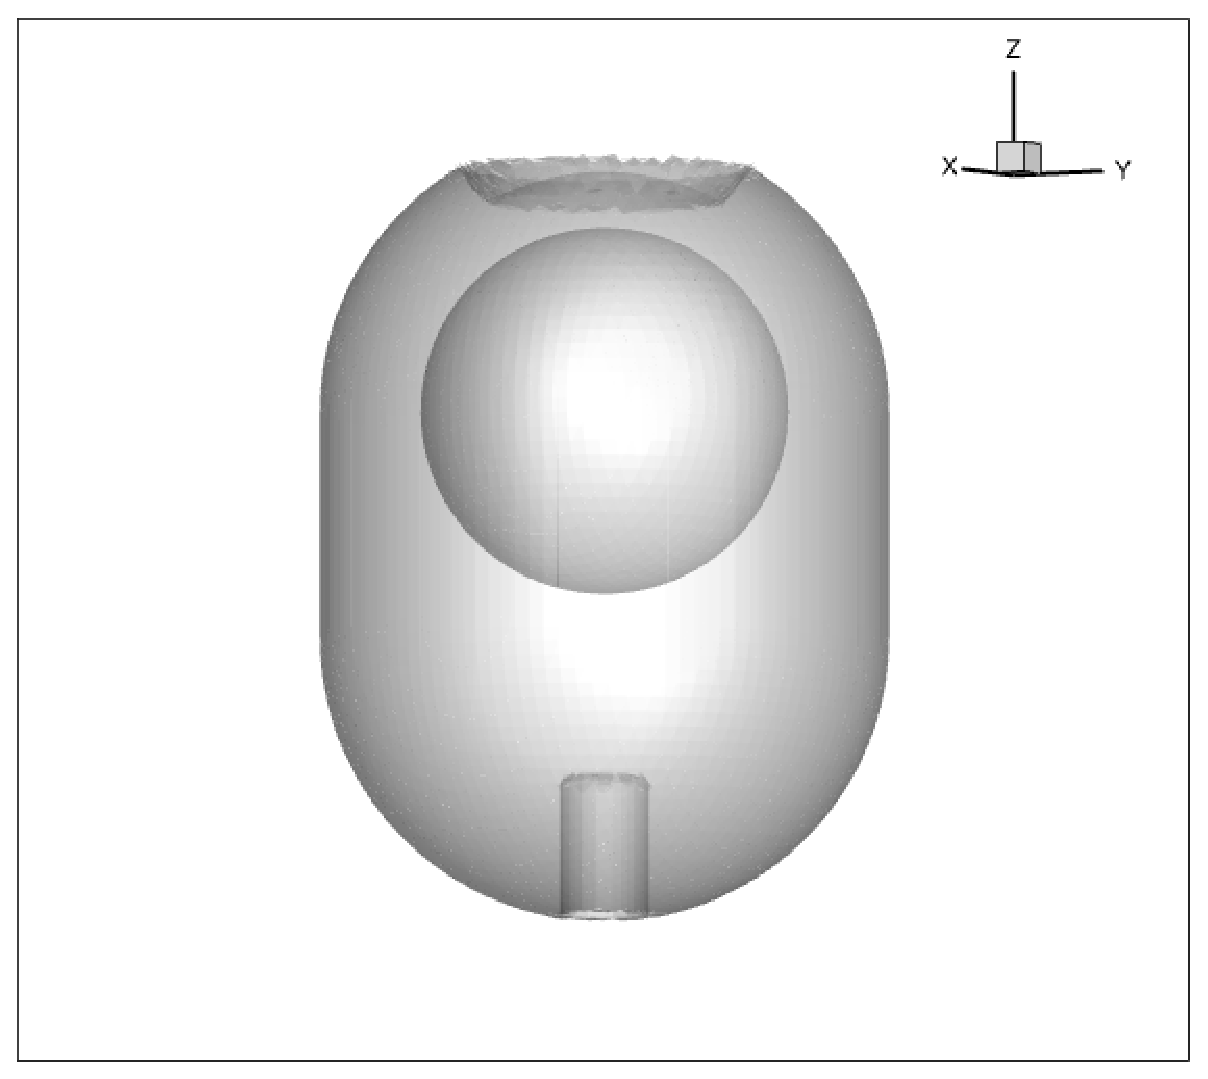
\includegraphics[width=0.3\textwidth]{3D_WEJ4p875_0.eps} 
		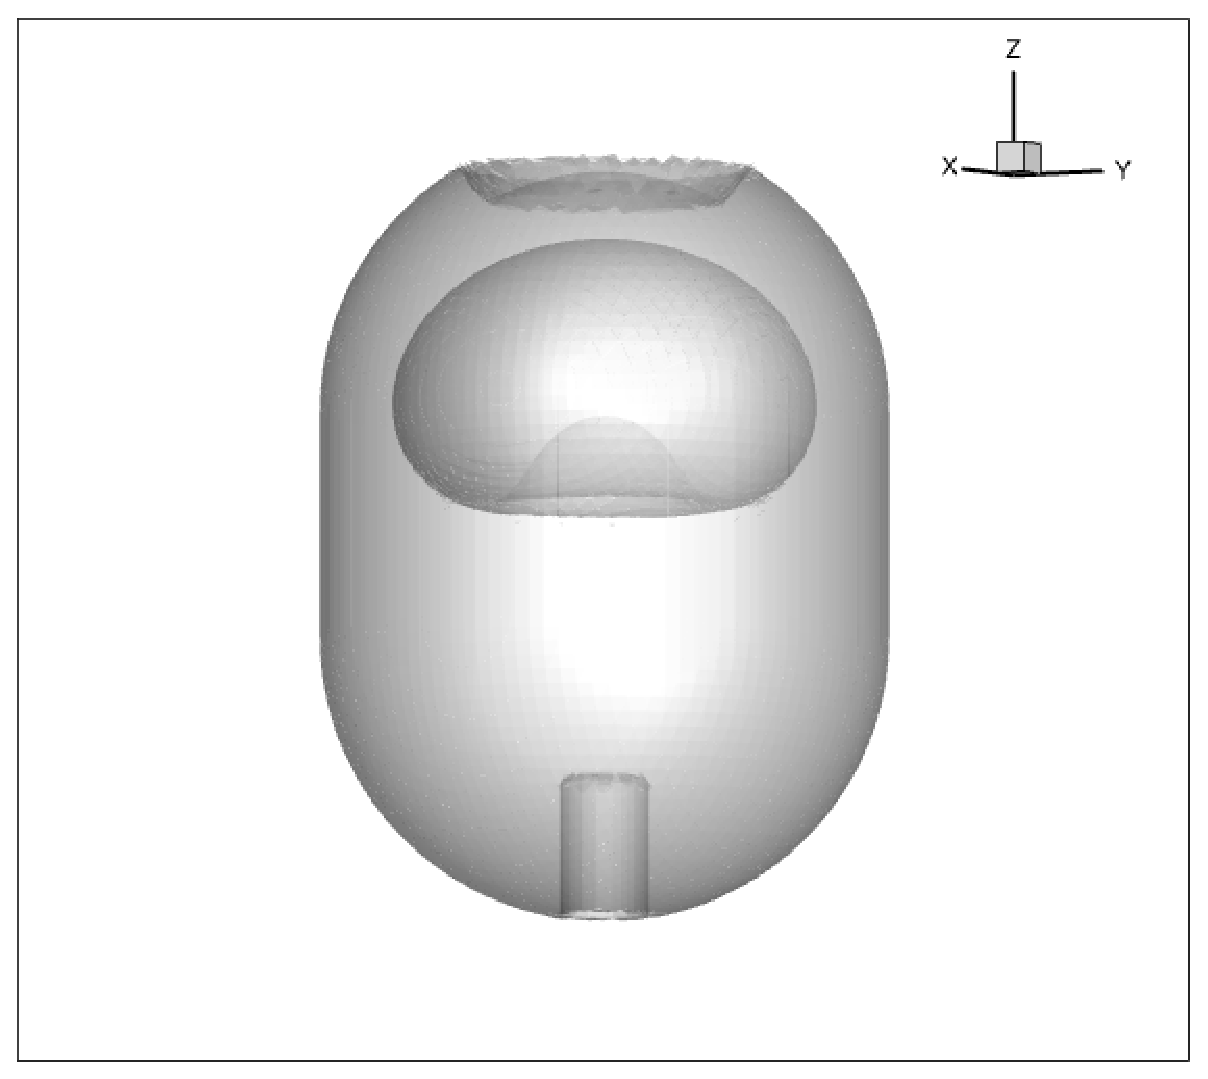
\includegraphics[width=0.3\textwidth]{3D_WEJ4p875_400.eps} 
		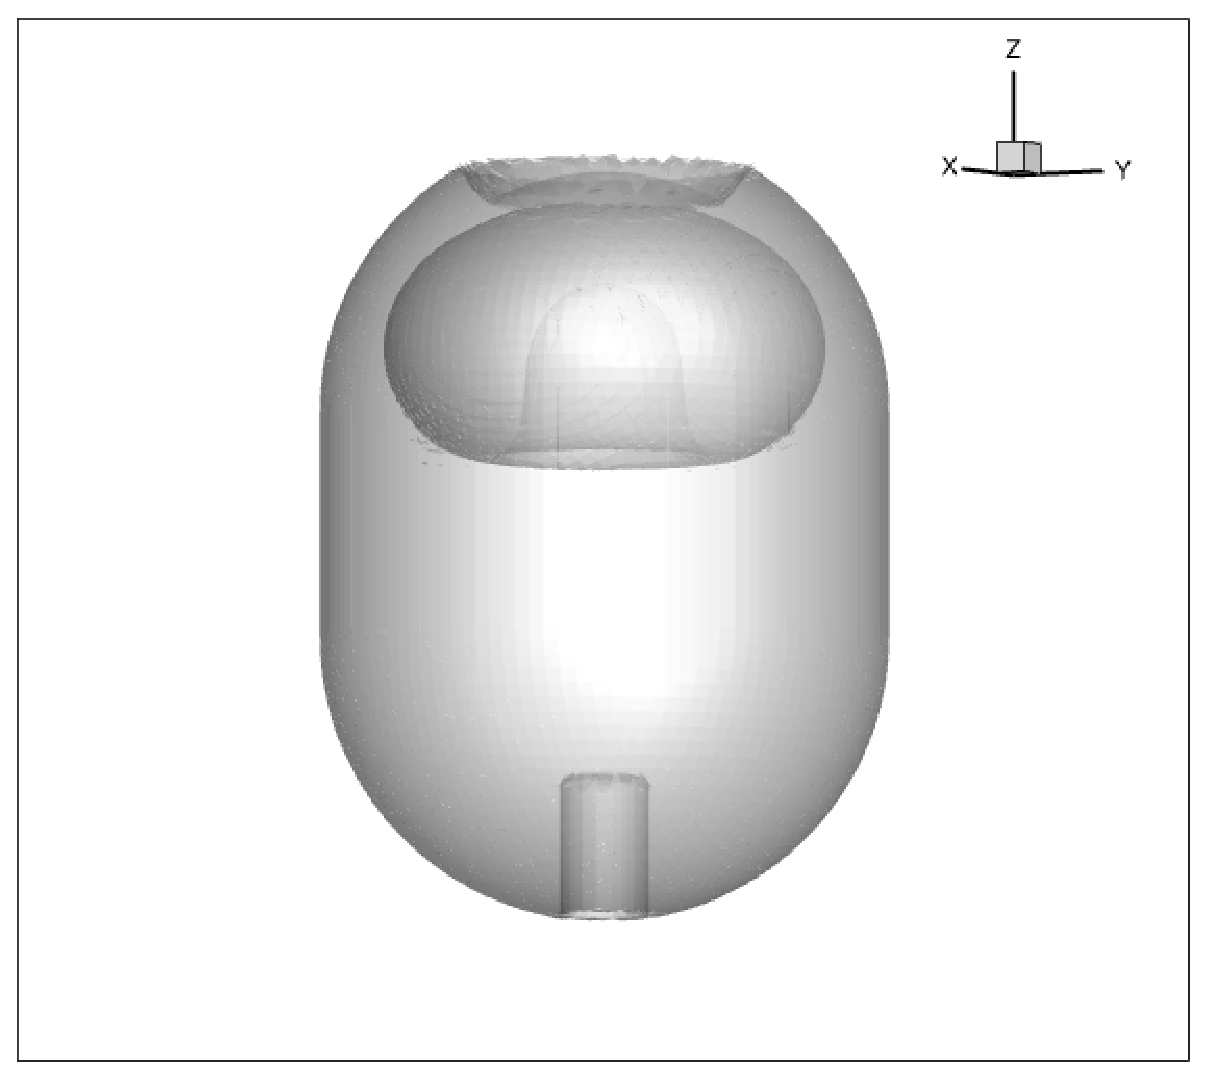
\includegraphics[width=0.3\textwidth]{3D_WEJ4p875_800.eps} 
		\caption{\textbf{CMOF}, deformation of a spherical ullage due to a liquid jet, $We_{j}=4.875$.  
			Times $t=0.0$, $8.45$, and $15.7$ shown.
			The jet does not penetrate the ullage.  Gridsize $64\times 64\times 64$. \textcolor{red}{add above, MOF non-penetrated ullage}}
		\label{3DWEJ4p875cmof}
	\end{minipage}
	\begin{minipage}[b]{1\linewidth}
		\centering
		\includegraphics[width=0.3\textwidth]{PMOFtankNoBreakup/PMOFtankNB_interface0000.png} 
		\includegraphics[width=0.3\textwidth]{PMOFtankNoBreakup/PMOFtankNB_interface0010.png} 
		\includegraphics[width=0.3\textwidth]{PMOFtankNoBreakup/PMOFtankNB_interface0020.png} 
		\caption{\textbf{PMOF}, deformation of a spherical ullage due to a liquid jet, $We_{j}=4.875$.  
			Times $t=0.0$, $8.45$, and $15.68$ shown.
			The jet does not penetrate the ullage.  Gridsize $64\times 64\times 64$. }
		\label{3DWEJ4p875plsmof}
	\end{minipage}
\end{figure}


\begin{figure}[H]
	\centering
	\begin{minipage}[b]{1\linewidth}
		\centering
		\includegraphics[width=0.3\textwidth]{jet2_mof1.png} 
		\includegraphics[width=0.3\textwidth]{jet2_mof2.png} 
		\includegraphics[width=0.3\textwidth]{jet2_mof3.png} 
		\vspace{-1em}
		\caption*{\textbf{MOF}: Times $t=0.0$, $7.84$, and $15.51$.}
		\label{3DWEJ5p25mof}
	\end{minipage}
	\begin{minipage}[b]{1\linewidth}
		\centering
		\includegraphics[width=0.3\textwidth]{jet2_cmof1.png} 
		\includegraphics[width=0.3\textwidth]{jet2_cmof2.png} 
		\includegraphics[width=0.3\textwidth]{jet2_cmof3.png} 
		\vspace{-1em}
		\caption*{\textbf{CMOF}: Times $t=0.0$, $7.84$, and $15.83$. }
		\label{3DWEJ5p25cmof}
	\end{minipage}
	\begin{minipage}[b]{1\linewidth}
		\centering
		\includegraphics[width=0.3\textwidth]{jet2_pmof1.png} 
		\includegraphics[width=0.3\textwidth]{jet2_pmof2.png} 
		\includegraphics[width=0.3\textwidth]{jet2_pmof3.png} 
		\vspace{-1em}
		\caption*{\textbf{PMOF}: Times $t=0.0$, $7.84$, and $15.60$.
			}
		\label{3DWEJ5p25plsmof}
	\end{minipage}
	\caption{Deformation of a spherical ullage due to a liquid jet, $We_{j}=5.25$. Grid size $64\times 64\times 64$. Jet penetrates ullage.}
\end{figure}

\begin{figure}[H]
	\centering
	\begin{minipage}[b]{0.49\linewidth}
		\centering
		\includegraphics[width=1\textwidth]{tank_reconst2d.png}
	\end{minipage}
	\begin{minipage}[b]{0.49\linewidth}
		\centering
		\includegraphics[width=1\textwidth]{tankLS_compare.png}
	\end{minipage}
	\caption{Comparison of vapor/liquid interface. Red: MOF, orange: CMOF, blue: PMOF. (\textbf{Left}) Reconstructed interface. (\textbf{Right}) Level set. \label{reconstLScompare}}
\end{figure} 


%% The Appendices part is started with the command \appendix;
%% appendix sections are then done as normal sections
\appendix
\section{Example Appendix Section}
\label{app1}

Appendix text.

%% For citations use: 
%%       \cite{<label>} ==> [1]

%%
%Example citation, See \cite{lamport94}.

%% If you have bib database file and want bibtex to generate the
%% bibitems, please use
%%
%%  \bibliographystyle{elsarticle-num} 
%%  \bibliography{<your bibdatabase>}

%% else use the following coding to input the bibitems directly in the
%% TeX file.

%% Refer following link for more details about bibliography and citations.
%% https://en.wikibooks.org/wiki/LaTeX/Bibliography_Management
\bibliographystyle{acm}
\bibliography{refs_plsmof}

%\begin{thebibliography}{00}
%% For numbered reference style
%% \bibitem{label}
%% Text of bibliographic item

%\bibitem{lamport94}
%  Leslie Lamport,
%  \textit{\LaTeX: a document preparation system},
%  Addison Wesley, Massachusetts,
%  2nd edition,
%  1994.

%\end{thebibliography}

\end{document}

\endinput
%%
%% End of file `elsarticle-template-num.tex'.
